\documentclass[10pt,a4paper]{article}
\usepackage[utf8]{inputenc}
\usepackage[italian]{babel}
\usepackage{amsmath}
\usepackage{amsfonts}
\usepackage{amssymb}
\usepackage{graphicx}
\usepackage[left=2cm,right=2cm,top=2cm,bottom=2cm]{geometry}
\newcommand{\rem}[1]{[\emph{#1}]}

\author{Gruppo AC \\ Federico Belliardo, Giulia Franchi, Francesco Mazzoncini}
\title{Esercitazione N.8: Oscillatore sinusoidale a ponte di Wien con OpAmp.}
\begin{document}
\maketitle
\section{Scopo dell'esperienza}
Lo scopo dell'esperienza è realizzare un oscillatore ad onda sinusoidale a ponte di Wien utilizzando un OpAmp.
\section{Montaggio del circuito e misura del loop gain}
Abbiamo montato il circuito in fig. \ref{oscillatore} utilizzando $R_1=$, $R_2=$, $R_3=$, $R_4=$, $R_5=$, un potenziometro con $P_{MAX}=$, due condensatori $C_1=$ e $C_2=$.
\begin{figure}[!htb]
  \centering
  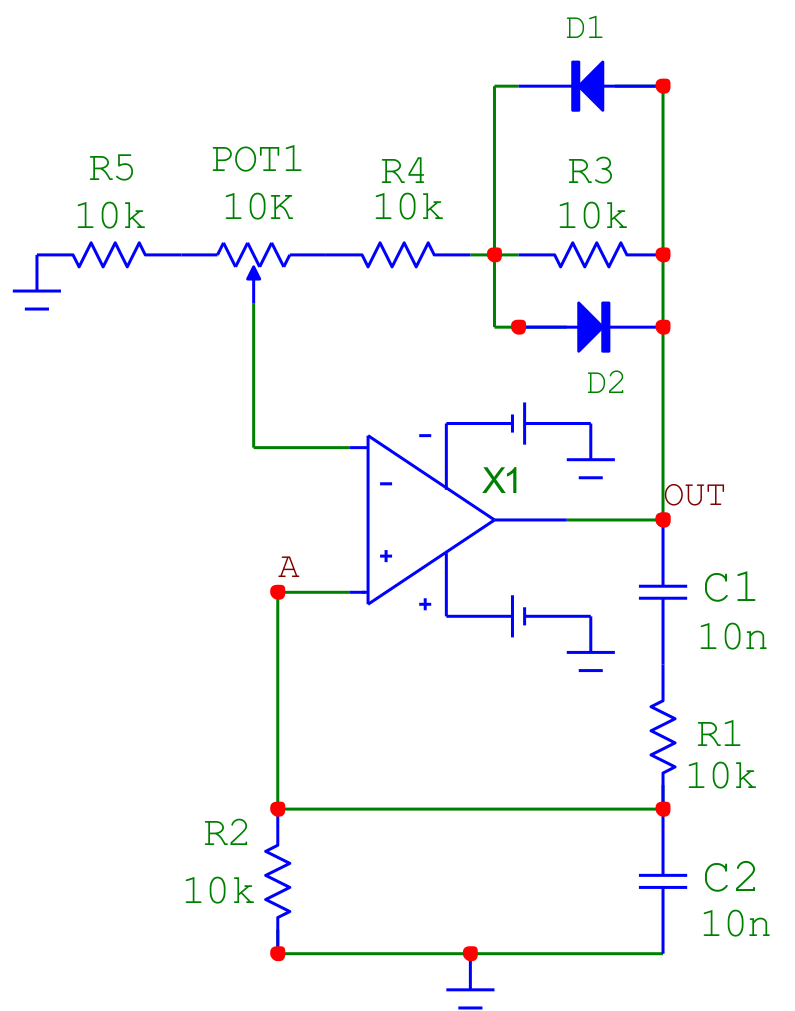
\includegraphics[scale=0.5]{pontediWien.png}
\caption{Circuito oscillatore a ponte di Wien.}
\label{oscillatore}
\end{figure}
Dal circuito si attendono quindi per i due sottocircuiti $R_1C_1$ e $R_2C_2$ le frequenze di taglio $f_1=\frac{1}{2 \pi R_1C_1}$ e $f_2=\frac{1}{2 \pi R_2C_2}$
Abbiamo scollegato il punto A dall'ingresso non invertente dell'OpAmp, inviando al suo posto attraverso il generatore di funzioni un segnale sinusoidale di ampiezza pari a circa $250\,mV$ con frequenza tra $500\,Hz$ e $3\,kHz$ \footnote{Da notare il fatto che l'intervallo considerato comprende anche la frequenza di taglio $f_1 \sim f_2$}
In tab.\ref{} abbiamo riportato i valori di $V_+$, $V_A$, del loro sfasamento $\phi$ e del loro rapporto $A_v=$. 
\rem{ INSERIRE TABELLA}
In seguito abbiamo riportato il diagramma di Bode dell'attenuazione e dello sfasamento in fig.\ref{} e fig.\ref{} rispettivamente.
\rem{eseguire fit dello sfasamento e verificare che si  $\phi$ si annulla per la frequenza di taglio dal fit, verificare in oltre che si ha il massimo del guadagno per la freq di taglio, ruotare infine il potenziometro per osservare la variazione di  $V_{OUT}$  e verificare la formula $A_v=\frac{R_3\parallel R_{diodo}+P_{MAX}+R_5}{\alpha P_{MAX}+R_5}$}


\section{Comportamento del circuito al variare del potenziometro}
Abbiamo sconnesso il generatore di funzioni e riconnesso il punto A all'ingresso non-invertente dell'OpAmp e abbiamo osservato il segnale in uscita al variare della resistenza del potenziometro, notando che:
\rem{Vedere cosa notiamo, fare attenzione alle piccole ampiezze (possibile rumore),notare quando otteniamo clipping}
\section{Misura della frequenza di oscillazione}
\rem{verificare che la frequenza di oscillazione sia proprio quella di taglio e vedere  ampiezze di alimentazioni basse per osservare  cambiamenti della frequenza dovuti al clipping}
\section{Misura del guadagno $A_v$ open loop}
Abbiamo impostato il potenziometro (ruotando la vite) in modo da raggiungere il punto di innesco dell’oscillazione e si è disconnesso il circuito di retroazione dall’ingresso non invertente, sostituendono con segnale sinusoidale di ampiezza  $V_+=$ emesso dal generatore di funzioni.
\rem{ misurare il segnale in uscita e ricavare il guadagno a loop aperto,confrontarlo con il valore teorico $A_v=3$ dovuto alla richieste che sia soddisfatta la condizione di Barkhausen $\beta \alpha =1$}
\section{Rimozione dei diodi}

\end{document}